%%%%%%%%%%%%%%%%%%%%%%%%%%%%%%%%%%%%%%%%%%%%%%%%%%%%%%%%%%%%%%%%
%%%%%%%%%%%%%%%%%%%%%%%%%%% Metadata %%%%%%%%%%%%%%%%%%%%%%%%%%%
%%%%%%%%%%%%%%%%%%%%%%%%%%%%%%%%%%%%%%%%%%%%%%%%%%%%%%%%%%%%%%%%
\documentclass{Axon}

\title{Discrete Mathematics and its Applications, 8th Edition - Chapter 1 The Foundations: Logic and Proofs - Section 1.2 Applications of Propositional Logic - Exercises}

\authors{
    \addauthor{Jeffrey G. Lind III}{jeffrey@jeffreylind.dev}
}

\addbibresource{Bibliography.bib}
%%%%%%%%%%%%%%%%%%%%%%%%%%%%%%%%%%%%%%%%%%%%%%%%%%%%%%%%%%%%%%%%
%%%%%%%%%%%%%%%%%%%%%%%%%%%%% Paper %%%%%%%%%%%%%%%%%%%%%%%%%%%%
%%%%%%%%%%%%%%%%%%%%%%%%%%%%%%%%%%%%%%%%%%%%%%%%%%%%%%%%%%%%%%%%
\begin{document}
\maketitle
\makeauthor
%%%%%%%%%%%%%%%%%%%%%%%%%%%%%%%%%%%%%%%%%%%%%%%%%%%%%%%%%%%%%%%%
%%%%%%%%%%%%%%%%%%%%%%%%%%% Abstract %%%%%%%%%%%%%%%%%%%%%%%%%%%
%%%%%%%%%%%%%%%%%%%%%%%%%%%%%%%%%%%%%%%%%%%%%%%%%%%%%%%%%%%%%%%%
\begin{abstract}
Notes on Discrete Mathematics and its Applications, 8th Edition - Chapter 1 The Foundations: Logic and Proofs - Section 1.2 Applications of Propositional Logic - Exercises \cite{Rosen}.
\end{abstract}
%%%%%%%%%%%%%%%%%%%%%%%%%%%%%%%%%%%%%%%%%%%%%%%%%%%%%%%%%%%%%%%%
%%%%%%%%%%%%%%%%%%%%%%%%%%% Section 1 %%%%%%%%%%%%%%%%%%%%%%%%%%
%%%%%%%%%%%%%%%%%%%%%%%%%%%%%%%%%%%%%%%%%%%%%%%%%%%%%%%%%%%%%%%%
\section*{}
In Exercises 1-6, translate the given statement into propositional logic using the propositions provided.

\section*{Exercise 1}
You cannot edit a protected Wikipedia entry unless you are an administrator. Express your answer in terms of \(e\): "You can edit a protected Wikipedia entry" and \(a\): "You are an administrator."

\noindent
\textbf{Solution:}
\(e \to a\)

\section*{Exercise 2}
You can see the movie only if you are over \(18\) years old or you have the permission of a parent. Express your answer in terms of \(m\): "You can see the movie," \(e\): "You are over \(18\) years old," and \(p\): "You have the permission of a parent."

\noindent
\textbf{Solution:}
\(m \to (e \lor p)\)

\section*{Exercise 3}
You can graduate only if you have completed the requirements of your major and you do not owe money to the university and you do not have an overdue library book. Express your answer in terms of \(g\): "You can graduate," \(m\): "You owe money to the university," \(r\): "You have completed the requirements of your major," and \(b\): "You have an overdue library book."

\noindent
\textbf{Solution:}
\(g \to (\lnot m \land r \land \lnot b)\)

\section*{Exercise 4}
To use the wireless network in the airport you must pay the daily fee unless you are a subscriber to the service. Express your answer in terms of \(w\): "You can use the wireless network in the airport," \(d\): "You pay the daily fee," and \(s\): "You are a subscriber to the service."

\noindent
\textbf{Solution:}
\(w \to (d \lor s)\)

\section*{Exercise 5}
You are eligible to be President of the U.S.A. only if you are at least 35 years old, were born in the U.S.A., or at the time of your birth both of your parents were citizens, and you have lived at least 14 years in the country. Express your answer in terms of \(e\): "You are eligible to be President of the U.S.A.," \(a\): "You are at least 35 years old," \(b\): "You were born in the U.S.A.," \(p\): "At the time of your birth, both of your parents were citizens," and \(r\): "You have lived at least 14 years in the U.S.A."

\noindent
\textbf{Solution:}
\(e \to (a \land (b \lor p) \land r)\)

\section*{Exercise 6}
You can upgrade your operating system only if you have a 32-bit processor running at 1 GHz or faster, at least 1 GB RAM, and 16GB free hard disk space, or a 64-bit processor running at 2 GHz or faster, at least 2 GB RAM, and at least 32 GB free hard disk space. Express your answer in terms of \(u\): "You can upgrade your operating system," \(b_{32}\): "You have a 32-bit processor," \(b_{64}\): "You have a 64-bit processor," \(g_1\): "Your processor runs at 1 GHz or faster," \(g_2\): "Your processor runs at 2 GHz or faster," \(r_1\): "Your processor has at least 2 GB RAM," \(h_{16}\): "You have at least 16 GB free hard disk space," and \(h_{32}\): "You have at least 32 GB free hard disk space.

\noindent
\textbf{Solution:}
\(u \to ((b_{32} \land g_1 \land r_1 \land h_{16}) \lor (b_{64} \land g_2\land r_2 \land h_{32}))\)

\section*{Exercise 7}
Express these system specifications using the propositions \(p\): "The message is scanned for viruses" and \(q\): "The message was sent from an unknown system" together with logical connectives (including negations).
\begin{enumerate}
    \item[\textbf{a)}][\textbf{a)}] "The message is scanned for viruses whenever the message was sent from an unknown system."
    \item[\textbf{b)}] "The message was sent from an unknown system but it was not scanned for viruses."
    \item[\textbf{c)}] "It is necessary to scan the message for viruses whenever it was sent from an unknown system."
    \item[\textbf{d)}] "When a message is not sent from an unknown system it is not scanned for viruses."
\end{enumerate}

\noindent
\textbf{Solution:}
\begin{enumerate}
    \item[\textbf{a)}] \(q \to p\)
    \item[\textbf{b)}] \(q \land \lnot p\)
    \item[\textbf{c)}] \(q \to p\)
    \item[\textbf{d)}] \(\lnot q \to \lnot p\)
\end{enumerate}

\section*{Exercise 8}
Express these system specifications using the propositions \(p\): "The user enters a valid password," \(q\): "Access is granted," and \(r\): "The user has paid the subscription fee" and logical connectives (including negations).
\begin{enumerate}
    \item[\textbf{a)}] "The user has paid the subscription fee, but does not enter a valid password."
    \item[\textbf{b)}] "Access is granted whenever the user has paid the subscription fee and enters a valid password."
    \item[\textbf{c)}] "Access is denied if the user has not paid the subscription fee."
    \item[\textbf{d)}] "If the user has not entered a valid password but has paid the subscription fee, then access is granted."
\end{enumerate}

\noindent
\begin{enumerate}
    \item[\textbf{a)}] \(r \land \lnot p\)
    \item[\textbf{b)}] \((p \land r) \to q\)
    \item[\textbf{c)}] \(\lnot r \to \lnot q\)
    \item[\textbf{c)}] \((\lnot p \land r) \to q\)
\end{enumerate}

\section*{Exercise 9}
Are these system specifications consistent? "The system is in a multiuser state if and only if it is operating normally. If the system is operating normally, the kernel is functioning. The kernel is not functioning or the system is in interrupt mode. If the system is not in multiuser state, then it is in interrupt mode. The system is not in interrupt mode."

\noindent
\textbf{Solution:}
Since the kernel is not functioning or the system is in interrupt mode, and the system is not in interrupt mode, then the kernel is not functioning. Since the kernel is not functioning, then the system is not operating normally. When the system is not operating normally, the system is not in multiuser state. However, it states that if the system is not in multiuser state, then it is in interrupt mode, a contradiction. Therefore, the system specifications are not consistent.

\section*{Exercise 10}
Are these system specifications consistent? "Whenever the system software is being upgraded, users cannot access the file system. If users can access the file system, then they can save new files. If users cannot save new files, then the system software is not being upgraded."

\noindent
\textbf{Solution:}
Whenever the system software is being upgraded, users cannot access the file system. However, the user not being able to access the file system does not imply that the user can not save new files. So although whenever users cannot save new files, the system software is not being upgraded, this does not contradict the first statement. Therefore, these system specifications are consistent.

\section*{Exercise 11}
Are these system specifications consistent? "The router can send packets to the edge system only if it supports the new address space. For the router to support the new address space it is necessary that the latest software release be installed. The router can send packets to the edge system if the latest software release is installed. The router does not support the new address space."

\noindent
\textbf{Solution:}
Since the router does not support the new address space, the router can not send packets to the edge system. Since the router can not send packets to the edge system, then the latest software release is not installed. IF the latest software release is installed, then the router supports the new address space. Since the router does not support the new address space and the latest software release is not installed, the system specifications are consistent.

\section*{Exercise 12}
Are these system specifications consistent? "If the file system is not locked, then new messages will be queued. If the file system is not locked, then the system is functioning normally, and conversely. If new messages are not queued, then they will be sent to the message buffer. If the file system is not locked, then new messages will be sent to the message buffer. New messages will not be sent to the message buffer."

\noindent
\textbf{Solution:}
Let \(p\): "The file system is locked," \(q\): "New messages are queued," \(r\): "The system if functioning normally," and \(s\): "Messages are sent to the message buffer."

Then, the system specifications are given as \(\lnot p \to q\), \(\lnot p \to r\), \(\lnot q \to s\), \(\lnot p \to s\), and \(\lnot s\).

Since \(\lnot s\), then we have \(p\) and \(q\). Then the first two statements do not contribute to any inconsistency. Therefore, the system specifications are consistent.

\section*{Exercise 13}
What Boolean search would you use to look for Web pages about beaches in New Jersey? What if you wanted to find Web pages about beaches on the isle of Jersey (in the English Channel)?

\noindent
\textbf{Solution:}
To look for Web pages about beaches in New Jersey, you would use the Boolean search: NEW \(AND\) JERSEY \(AND\) BEACHES. To find Web pages about beaches on the isle of Jersey, you would use the Boolean search: (JERSEY \(AND\) BEACHES) \(NOT\) NEW.

\section*{Exercise 14}
What Boolean search would you use to look for Web pages about hiking in West Virginia? What if you wanted to find Web pages about hiking in Virginia, but not in West Virginia?

\noindent
\textbf{Solution:}
To look for Web pages about hiking in West Virginia, you would use the Boolean search: WEST \(AND\) VIRGINIA \(AND\) HIKING. To find Web pages about hiking in Virginia, but not in West Virginia, you would use the Boolean search: (VIRGINIA \(AND\) HIKING) \(NOT\) WEST.

\section*{Exercise 15}
What Google search would you use to look for Web pages relating to Ethiopian restaurants in New York or New Jersey?

\noindent
\textbf{Solution:}
To search Google for Web pages relating to Ethiopian restaurants in New York or New Jersey, you would use: "ETHIOPIAN RESTAURANTS" \(AND\) ("NEW YORK" \(OR\) "New Jersey").

\section*{Exercise 16}
What Google search would you use to look for men's shoes or boots not designed for work?

\noindent
\textbf{Section:}
The Google search you would use to look for men's shoes or boots not designed for work is MEN'S (SHOES \(OR\) BOOTS) - WORK.

\section*{Exercise 17}
Suppose that in Example 7, the inscriptions on Trunks 1, 2, and 3 are "The treasure is in Trunk 3," "The treasure is in Trunk 1," and "This trunk is empty." For each of these statements, determine whether the Queen who never lies could state this, and if so, which trunk the treasure is in.
\begin{enumerate}
    \item[\textbf{a)}] "All the inscriptions are false."
    \item[\textbf{b)}] "Exactly one of the inscriptions is true."
    \item[\textbf{c)}] "Exactly two of the inscriptions are true."
    \item[\textbf{d)}] "All three inscriptions are true."
\end{enumerate}

\noindent
\textbf{Solution:}
\begin{enumerate}
    \item[\textbf{a)}] Suppose that the Queen states "All the inscriptions are false." Therefore, Trunk 1 would entail that the treasure is not in Trunk 3. Then, Trunk 2 would entail that the treasure is not in Trunk 1. Finally, Trunk 3 would entail that Trunk 3 contains the treasure, a contradiction. Therefore, the Queen could not state this.
    
    \item[\textbf{b)}] Suppose that the Queen states "Exactly one of the inscriptions is true." Suppose that Trunk 1's inscription is true. Then, we have Trunks 1, 2, and 3 entailing that the treasure is in Trunk 3, the treasure is not in Trunk 1, and that Trunk 3 is not empty, a consistent set of statements. Therefore, the Queen can state that "Exactly one of the inscriptions is true." However, the location of the treasure cannot be determined.
    
    \item[\textbf{c)}] Suppose that the Queen states "Exactly two of the inscriptions are true."

    Suppose that the inscriptions on Trunks 1 and 2 are true. Then, Trunks 1 and 2 would entail that the treasure is in Trunk 3 and that the treasure is in Trunk 1, a contradiction.

    Suppose that the inscriptions on Trunks 1 and 3 are true. Then, Trunks 1, 2, and 3 would entail that the treasure is in Trunk 3, the treasure is not in Trunk 1, and that Trunk 3 is empty, a contradiction.

    Suppose that the inscriptions on Trunks 2 and 3 are true. Then, Trunks 1, 2, and 3 would entail that the treasure is not in Trunk 3, the treasure is in Trunk 1, and that Trunk 3 is empty. This is valid, and thus the Queen could state that "Exactly two of the inscriptions are true." The treasure is in Trunk 1.
    
    \item[\textbf{d)}] Suppose that the Queen states "All three inscriptions are true." This gives a contradiction due to the inscriptions on Trunks 1 and 2.
\end{enumerate}

\section*{Exercise 18}
Suppose that in Example 7 there are treasures in two of the three trunks. The inscriptions on Trunks 1, 2, and 3 are "This trunk is empty," "There is a treasure in Trunk 1," and "There is a treasure in Trunk 2." For each of these statements, determine whether the Queen who never lies could state this, and if so, which two trunks the treasures are in.
\begin{enumerate}
    \item[\textbf{a)}] "All the inscriptions are false."
    \item[\textbf{b)}] "Exactly one of the inscriptions is true."
    \item[\textbf{c)}] "Exactly two of the inscriptions are true."
    \item[\textbf{d)}] "All three inscriptions are true."
\end{enumerate}

\noindent
\textbf{Solution:}
\begin{enumerate}
    \item[\textbf{a)}] Suppose that the Queen states "All the inscriptions are false."

    Then, Trunks 1, 2, and 3 would entail that Trunk 1 is not empty, there is not a treasure in Trunk 1, and there is not a treasure in Trunk 2, a contradicting set of statements. Therefore, the Queen can not state "All the inscriptions are false."
    
    \item[\textbf{b)}] Suppose that the Queen states "Exactly one of the inscriptions is true."

    Suppose that Trunk 1 is true. Then Trunks 1, 2, and 3 would entail that Trunk 1 is empty, there is not a treasure in Trunk 1, and there is not a treasure in Trunk 2. This only leaves the possibility for one Trunk to contain the treasure, which is not possible.

    Suppose that Trunk 2 is true. Then Trunks 1, 2, and 3 would entail that Trunk 1 is not empty, there is a treasure in Trunk 1, and there is not a treasure in Trunk 2. This is a valid set of statements, thus the Queen can state "Exactly one of the inscriptions is true," and the treasures are in Trunks 1 and 3.
    
    \item[\textbf{c)}] Suppose that the Queen states "Exactly two of the inscriptions are true."

    Suppose that the inscriptions on Trunks 1 and 2 are true. Then Trunks 1, 2, and 3 would entail that Trunk 1 is empty, there is a treasure in Trunk 1, and there is not a treasure in Trunk 2, a contradictory set of statements.

    Suppose that the inscriptions on Trunks 1 and 3 are true. Then Trunks 1, 2, and 3 would entail that Trunk 1 is empty, there is not a treasure in Trunk 1, and there is a treasure in Trunk 2. This is a valid set of statements, and thus the Queen can state "Exactly two of the inscriptions are true." If this were to be the case, the treasures would be in Trunks 2 and 3.

    Suppose that the inscriptions on Trunks 2 and 3 are true. Then Trunks 1, 2, and 3 would entail that Trunk 1 is not empty, there is a treasure in Trunk 1, and there is a treasure in Trunk 2. This is a valid set of statements and the treasures would be in Trunks 1 and 2. This ambiguity between the valid sets of combinations of statements implies that the treasures' location can not be determined.
    
    \item[\textbf{d)}] Suppose that the Queen states "All three inscriptions are true."

    Then, Trunks 1, 2, and 3 entail that Trunk 1 is empty, there is a treasure in Trunk 1, and there is a treasure in Trunk 2, a contradictory set of statements.
\end{enumerate}

\section*{Exercise 19}
Each inhabitant of a remote village always tells the truth or always lies. A villager will give only a "Yes" or a "no" response to a question a tourist asks. Suppose you are a tourist visiting this area and come to a fork in the road. One branch leads to the ruins you want to visit; the other branch leads deep into the jungle. A villager is standing at the fork in the road. What one question can you ask the villager to determine which branch to take?

\noindent
\textbf{Solution:}
If you simply ask if the right fork leads you to the ruins that you want to visit, the villager can tell you "Yes" or "No," but can also be telling the truth or lying, so a question of this form is not sufficient.

Suppose you asked a question of the form "If I were to ask you whether the right branch leads to the ruins, would you answer yes?" If the villager says no, he is not telling you the truth, then that would be contradictory, as he can't both be telling the truth and saying that he is not telling the truth. If the villager says yes, he is telling the truth, then you can ensure that the villager will correctly tell you if the right fork is the fork to the ruins. If he says "Yes," take the right fork, and if he says "No," take the left fork.

\section*{Exercise 20}
An explorer is captured by a group of cannibals. There are two types of cannibals --- those who always tell the truth and those who always lie. The cannibals will barbecue the explorer unless he can determine whether a particular cannibal always lies or always tells the truth. He is allowed to ask the cannibal exactly one question.
\begin{enumerate}
    \item[\textbf{a)}] Explain why the question "Are you a liar?" does not work.
    \item[\textbf{b)}] Find a question that the explorer can use to determine whether the cannibal always lies or always tells the truth.
\end{enumerate}

\noindent
\textbf{Solution:}
\begin{enumerate}
    \item[\textbf{a)}] Suppose you ask a liar cannibal if they are a liar. Then, the cannibal will answer "No," that they are telling the truth. If you ask a true cannibal if they are a liar, they will also respond "No." Therefore, this question can not be used to determine whether a cannibal is a liar or not.
    \item[\textbf{b)}] Ask the cannibal whether \(2 + 2 = 4\). If the cannibal responds yes, then the cannibal is telling the truth. If the cannibal responds no, then the cannibal is a liar.
\end{enumerate}

\section*{Exercise 21}
When three professors are seated in a restaurant, the hostess asks them: "Does everyone want coffee?" The first professor says "I do not know." The second professor then says "I do not know." Finally, the third professor says "No, not everyone wants coffee." The hostess comes back and gives coffee to the professors who want it. How did she figure out who wanted coffee?

\noindent
\textbf{Solution:}
Since the third professor says "No, not everyone wants coffee," there are only 2 professors who want coffee: professors 1 and 2, 1 and 3, or 2 and 3. Since the first professor says he does not know if everyone wants coffee, that implies that he wants coffee, because him not wanting coffee would mean that not everyone wants coffee. This is the same case for second professor. Therefore, professors 1 and 2 want coffee, and professor 3 does not want coffee.

\section*{Exercise 22}
When planning a party you want to know whom to invite. Among the people you would like to invite are three touchy friends. You know that if Jasmine attends, she will become unhappy if Samir is there, Samir will attend only if Kanti will be there, and Kanti will not attend unless Jasmine also does. Which combinations of these three friends can you invite so as not to make someone unhappy?

\noindent
\textbf{Solution:}
Let \(j\), \(s\), and \(k\) be propositions that Jasmine, Samir, and Kanti attend. Then, the three statements can be translated as
\begin{itemize}
    \item \(j \to \lnot s\),
    \item \(s \to k\),
    \item \(k \to j\).
\end{itemize}

Suppose \(j\), so then \(\lnot s\). Despite \(\lnot s\), we can still have \(k\). Thus we can have Jasmine, or Jasmine and Kanti attend.

Suppose \(s\), so then \(k\). But if \(k\), then we must have \(j\). However, this gives a contradiction.

Suppose \(k\), so then \(j\). But \(j \to \lnot s\), so we can again have Jasmine or Kanti.

Therefore, we can only have Jasmine, or Jasmine and Kanti.

\section*{}
Exercises 23-27 relate to inhabitants of the island of knights and knaves created by Smullyan, where knights always tell the truth and knaves always lie. You encounter two people, \(A\) and \(B\). Determine, if possible, what \(A\) and \(B\) are if they address you in the ways described. If you cannot determine what these two people are, can you draw any conclusions?

\section*{Exercise 23}
\(A\) says "At least one of us is a knave" and \(B\) says nothing.

\noindent
\textbf{Solution:}
Suppose \(A\) is a knave. When \(A\) says "At least one of us is a knave," this contradicts the assumption that \(A\) is a knave, because \(A\) is telling the truth. Therefore, \(A\) is not a knave and is a knight.

If \(A\) is a knight and says "At least one of us is a knave," then that leaves \(B\) to be a knave. Therefore, \(A\) is a knight and \(B\) is a knave.

\section*{Exercise 24}
\(A\) says "The two of us are both knights" and \(B\) says "\(A\) is a knave."

\noindent
\textbf{Solution:}
Suppose \(A\) is a knave. Then when \(A\) says "The two of us are both knights," he implies that the two of them are not both knights. When \(B\) says "\(A\) is a knave," this coheres to what \(A\) says. Therefore, \(A\) is a knave and \(B\) is a knight.

\section*{Exercise 25}
\(A\) says "I am a knave or \(B\) is a knight" and \(B\) says nothing.

\noindent
\textbf{Solution:}
Suppose \(A\) is a knave. Then when \(A\) says "I am a knave or \(B\) is a knight," he entails the negation which is "I am a knight and \(B\) is a knave." This is contradictory.

Suppose \(A\) is a knight. Then when \(A\) says "I am a knave or \(B\) is a knight," \(B\) must also be a knight. Therefore, \(A\) and \(B\) are both knights.

\section*{Exercise 26}
Both \(A\) and \(B\) say "I am a knight."

\noindent
\textbf{Solution:}
Suppose \(A\) is a knave. Then it is possible for \(B\) to be a knave or knight.

Suppose \(A\) is a knight. Then it is possible for \(B\) to be a knave or knight.

Therefore, all combinations are possible.

\section*{Exercise 27}
\(A\) says "We are both knaves" and \(B\) says nothing.

\noindent
\textbf{Solution:}
Suppose \(A\) is a knight. Then when \(A\) says "We are both knaves," he is contradicting this assumption. Therefore \(A\) must not be a knight.

Suppose \(A\) is a knave. Then when \(A\) says "We are both knaves," he implies that not both of them are knaves, i.e. \(B\) is not a knave. Therefore, \(A\) is a knave and \(B\) is a knight.

\section*{}
Exercises 28-35 relate to inhabitants of an island on which there are three kinds of people: knights who always tell the truth, knaves who always lie, and spies (called normals by Smullyan [Sm78]) who can either lie or tell the truth. You encounter three people, \(A\), \(B\), and \(C\). You know one of these people is a knight, one is a knave, and one is a spy. Each of the three people knows the type of person each of the other two is. For each of these situations, if possible, determine whether there is a unique solution and determine who the knave, knight, and spy are. When there is no unique solution, list all possible solutions or state that there are no solutions.

\section*{Exercise 28}
\(A\) says "\(C\) is the knave," \(B\) says "\(A\) is the knight," and \(C\) says "I am the spy."

\noindent
\textbf{Solution:}
Suppose \(A\) is a knight. Then \(C\) is a knave. Finally, \(B\) must be a spy. This is a valid combination.

Suppose \(A\) is a knave. Then, \(C\) is not a knave and must be a spy. Finally, \(B\) must be a knight, but this gives a contradiction.

Suppose \(A\) is a spy. Then \(C\) must be a knave. Finally, \(B\) must be a knight, but this gives a contradiction.

Therefore, \(A\) is a knight, \(C\) is a knave, and \(B\) is a spy.

\section*{Exercise 29}
\(A\) says "I am the knight," \(B\) says "I am the knave," and \(C\) says "\(B\) is the knight."

\noindent
\textbf{Solution:}
Suppose \(B\) is a knight. This gives a contradiction, so \(B\) is not a knight.

Suppose \(B\) is a knave. Again, this gives a contradiction, so \(B\) must be a spy.

Suppose \(B\) is a spy and \(A\) is a knight. Then, \(C\) must be a knave. This combination is valid.

Suppose \(B\) is a spy and \(A\) is a knave. Then, \(C\) must be a knight, which gives a contradiction. Therefore, this combination is invalid.

Therefore, \(B\) is a spy, \(A\) is a knight, and \(C\) is a knave.

\section*{Exercise 30}
\(A\) says "I am the knave," \(B\) says "I am the knave," and \(C\) says "I am the knave."

\noindent
\textbf{Solution:}
By reasoning of Exercise 28, \(A\), \(B\), and \(C\) must all be spies, which is not possible. Therefore, there are no solutions.

\section*{Exercise 31}
\(A\) says "I am the knight," \(B\) says "\(A\) is telling the truth," and \(C\) says "I am the spy."

\noindent
\textbf{Solution:}
Suppose \(A\) is a knight. Then, \(B\) must be a spy. Finally, \(C\) must be a knave.

Suppose \(A\) is a knave. Then, \(B\) must be a spy. Finally, \(C\) must be a knight, which gives a contradiction.

Suppose \(A\) is a spy. Then, \(B\) must be a knave. Finally, \(C\) must be a knight, which gives a contradiction.

Therefore, \(A\) is a knight, \(B\) is a spy, and \(C\) is a knave.

\section*{Exercise 32}
\(A\) says "I am the knight," \(B\) says "\(A\) is not the knave," and \(C\) says "\(B\) is not the knave."

\noindent
\textbf{Solution:}
Suppose \(A\) is a knight. Then \(B\) must be a spy, and \(C\) must be a knave, a contradiction.

Suppose \(B\) is a knight. Then, \(A\) must be the spy, and \(C\) must be a knave, a contradiction.

Suppose \(C\) is a knight. Then, \(B\) must be a spy, and \(A\) must be a knave.

Therefore, \(C\) is a knight, \(B\) is a spy, and \(A\) is a knave.

\section*{Exercise 33}
\(A\) says "I am the knight," \(B\) says "I am the knight," and \(C\) says "I am the knight."

\noindent
\textbf{Solution:}
Suppose \(A\) is a knight. Then, \(B\) can by a spy and \(C\) can be a knave, or \(B\) can be a knave and \(C\) can be a spy.

Therefore, there are no unique solutions to this problem.

\section*{Exercise 34}
\(A\) says "I am not the spy," \(B\) says "I am not the spy," and \(C\) says "\(A\) is the spy."

\noindent
\textbf{Solution:}
Suppose \(A\) is a knight. Then, \(B\) must be a spy and \(C\) can be a knave.

Suppose \(B\) is a knight. Then, \(A\) must be a knave, a contradiction.

Suppose \(C\) is a  knight. Then, \(A\) must be a spy, but \(B\) must be a knave, a contradiction.

Therefore, \(A\) is a knight, \(B\) is a spy, and \(C\) is a knave.

\section*{Exercise 35}
\(A\) says "I am not the spy," \(B\) says "I am not the spy," and \(C\) says "I am not the spy."

\noindent
\textbf{Solution:}
Suppose \(A\) is a knight. Then there are no further possibilities as either \(B\) or \(C\) would have to be a knave, a contradiction.

This same argument applies to all possibilities. Therefore, there is no solution.

\section*{}
Exercises 36-42 are puzzles that can be solved by translating statements into logical expressions and reasoning from these expressions using truth tables.

\section*{Exercise 36}
The police have three suspects for the murder of Mr. Cooper: Mr. Smith, Mr. Jones, and Mr. Williams. Smith, Jones, and Williams each declare that they did not kill Cooper. Smith also states that Cooper was a friend of Jones and that Williams disliked him. Jones also states that he did not know Cooper and that he was out of town the day Cooper was killed. Williams also states that he saw both Smith and Jones with Cooper the day of the killing and that either Smith or Jones must have killed him. Can you determine who the murderer was if
\begin{enumerate}
    \item[\textbf{a)}] one of the three men is guilty, the two innocent men are telling the truth, but the statements of the guilty man may or may not be true?
    \item[\textbf{b)}] innocent men do not lie?
\end{enumerate}

\noindent
\textbf{Solution:}
The problem statement gives the following statements:
\begin{itemize}
    \item Smith, Jones, and Williams each declare that they did not kill Cooper.
    \item Smith states that Cooper was a friend of Jones and that Williams disliked him.
    \item Jones states that he did not know Cooper and that he was out of town the day Cooper was killed.
    \item Williams states that he saw both Smith and Jones with Cooper the day of the killing and that either Smith or Jones must have killed him.
\end{itemize}
\begin{enumerate}
    \item[\textbf{a)}]
    Suppose that Smith killed Cooper, so Jones and Williams must be telling the truth. This causes a contradiction, as Jones states that he did not know Cooper, but William states that he saw Jones with Cooper. Thus, Smith did not kill Cooper.

    Suppose that Williams killed Cooper, so Smith and Jones must be telling the truth. This causes a contradiction, as Smith states that Cooper and Jones were friends, but Jones states that he did not know Cooper. Thus, Williams did not kill Cooper.

    Therefore, since there was one guilty man, Jones must have killed Cooper.
    
    \item[\textbf{b)}]
    Since we only know that innocent men do not lie, there can be 0, 1, 2, or 3 guilty men.

    If there are 0 guilty men, then Smith, Jones, and Williams must all be telling the truth. This causes a contradiction, as Smith states that Jones and Cooper were friends, but Jones states that he did not know Cooper. Therefore, there can not be 0 guilty men.
    
    If there is 1 guilty man, then by part a), we know that Jones must have killed Cooper.

    If there are 2 guilty men, then either Smith and Jones, Jones and Williams, or Smith and Williams must be guilty.
    
    Suppose that Smith and Jones are guilty, thus Williams is telling the truth. This coincides with his statement, and is thus a possibility.
    
    Suppose that Jones and Williams are guilty, thus Smith is telling the truth. This coincides with his statement, and is thus a possibility.

    Suppose that Smith and Williams are guilty, thus Jones is telling the truth. This coincides with his statement, and is thus a possibility.

    Therefore, everything is possible if there are 2 guilty men.

    It is also possible that all 3 men are guilty.
\end{enumerate}

\section*{Exercise 37}
Steve would like to determine the relative salaries of three coworkers using two facts. First, he knows that if Fred is not the highest paid of the tree, then Janice is. Second, he knows that if Janice is not the lowest paid, then Maggie is paid the most. Is it possible to determine the relative salaries of Fred, Maggie, and Janice from what Steve knows? If so, who is paid the most and who the least? Explain your reasoning.

\noindent
\textbf{Solution:}
The problem description gives the following statements:
\begin{itemize}
    \item If Fred is not the highest paid of the three, then Janice is.
    \item If Janice is not the lowest paid, then Maggie is paid the most.
\end{itemize}
Let \(p\), \(q\), \(r\), and \(s\) be the propositions "Fred is the highest paid," "Janice is the highest paid," "Janice is the lowest paid," and "Maggie is the highest paid."

Then, the statements can be formalized as
\begin{itemize}
    \item \(\lnot p \to q\) 
    \item \(\lnot r \to s\)
\end{itemize}
Additionally, only one person can be the highest paid, so the compound propositions \(p \oplus q \oplus s\) holds true.

Suppose that Fred is not the highest paid of the three. Then, Janice must be the highest paid of the three. Janice not being the lowest paid follows from this, and thus Maggie is paid the most. This is a contradiction, and so Fred is the highest paid of the three.

Since we know that if Janice is not the lowest paid, then Maggie is paid the most, then Janice must be the lowest paid. Therefore, the order of decreasing pay is Fred, Maggie, and Janice.

\section*{Exercise 38}
Five friends have access to a chat room. Is it possible to determine who is chatting if the following information is known? Either Kevin or Heather, or both, are chatting. Either Randy or Vijay, but not both, are chatting. If Abby is chatting, so is Randy. Vijay and Kevin are either both chatting or neither is. If Heather is chatting, then so are Abby and Kevin. Explain your reasoning.

\noindent
\textbf{Solution:}
The problem description gives the following statements:
\begin{itemize}
    \item Either Kevin or Heather, or both, are chatting.
    \item Either Randy or Vijay, but not both, are chatting.
    \item If Abby is chatting, so is Randy.
    \item Vijay and Kevin are either both chatting or neither is.
    \item If Heather is chatting, then so are Abby and Kevin.
\end{itemize}

Suppose that Heather is chatting. Then, Abby and Kevin must be chatting. If Abby is chatting, then so is Randy. But then Vijay can't be chatting, and thus neither is. A contradiction. Thus, Heather is not chatting.

Suppose that Abby is chatting. Then, Randy must be chatting. Then, Vijay is not chatting. Then, Kevin is not chatting. Then, since either Kevin or Heather, or both, are chatting, then Heather must be chatting. However, if Heather is chatting, then so are Abby and Kevin, a contradiction. Thus, Abby is not chatting.

Suppose that Vijay is chatting. Then, Kevin must also be chatting. Since Vijay is chatting, then Randy must not be chatting. We know that Heather nor Abby can be chatting. This poses no contradictions, so therefore Vijay is chatting.

Since Vijay is chatting, then Kevin must also be chatting.

Since Vijay is chatting, then Randy can't be chatting. 

Therefore, only Vijay and Kevin are chatting.

\section*{Exercise 39}
A detective has interviewed four witnesses to a crime. From the stories of the witnesses the detective has concluded that if the butler is telling the truth then so is the cook; the cook and the gardener cannot both be telling the truth; the gardener and the handyman are not both lying; and if the handyman is telling the truth then the cook is lying. For each of the four witnesses, can the detective determine whether that person is telling the truth or lying? Explain your reasoning.

\noindent
\textbf{Solution:}
The problem description gives the following statements:
\begin{itemize}
    \item If the butler is telling the truth then so is the cook.
    \item The cook and the gardener cannot both be telling the truth.
    \item The gardener and the handyman are not both lying.
    \item If the handyman is telling the truth then the cook is lying.
\end{itemize}

Butler = nil
Cook = nil
Gardener
Handyman

Suppose that the butler is telling the truth. Then, the cook must also be telling the truth. Since the cook and the gardener cannot both be telling the truth, then the gardener is lying. Since the gardener and the handyman are not both lying, then the handyman must be telling the truth. However if the handyman is telling the truth, then the cook is lying, a contradiction. Thus, the butler is not telling the truth.

Suppose that the cook is telling the truth. Then, the gardener is lying. Then, the handyman must be telling the truth. However since the handyman is telling the truth, then the cook is lying, a contradiction. Therefore the cook is not telling the truth.

Suppose that the gardener is telling the truth. Then, the cook must be lying. However, the handyman can also be telling the truth or lying and cause no contradictions, and thus the detective can conclude that the butler and cook are lying, but cannot determine the state of the gardener and handyman.

\section*{Exercise 40}
Four friends have been identified as suspects for an unauthorized access into a computer system. They have made statements to the investigating authorities. Alice said, "Carlos did it." John said, "I did not do it." Carlos said, "Diana did it." Diana said, "Carlos lied when he said that I did it."
\begin{enumerate}
    \item[\textbf{a)}] If the authorities also know that exactly one of the four suspects is telling the truth, who did it? Explain your reasoning.
    \item[\textbf{b)}] If the authorities also know that exactly one is lying, who did it? Explain your reasoning.
\end{enumerate}

\noindent
\textbf{Solution:}
The problem description gives the following statements:
\begin{itemize}
    \item Alice said, "Carlos did it."
    \item John said, "I did not do it."
    \item Carlos said, "Diana did it."
    \item Diana said, "Carlos lied when he said that I did it."
\end{itemize}

\begin{enumerate}
    \item[\textbf{a)}] Suppose that exactly one of the suspects is telling the truth.
    
    Suppose that Alice is telling the truth. Then, John, Carlos, and Diana must be lying. John said that he did not do it, a lie, and thus he did it. However, this contradicts Alice's statement, a contradiction. Thus, Alice is not telling the truth
    
    Suppose that John is telling the truth. Then, Alice, Carlos, and Diana must be lying. Alice said that Carlos did it, and thus Carlos did not do it. Carlos said that Diana did it, and thus Diana did not do it. Diana said that Carlos lied when he said that I did it, and thus Carlos did not lie, a contradiction. Thus, John is not telling the truth.

    Suppose that Carlos is telling the truth. Then, Alice, John, and Diana must be lying. Diana said that Carlos lied when he said that Diana did it, so then Carlos did not lie and Diana did it. This would make John's statement truthful however, a contradiction. Therefore Carlos is not telling the truth.

    Thus, Diana is telling the truth and John did it.
    
    \item[\textbf{b)}] Suppose that exactly one of the suspects is lying.

    Alice = T
    John = T
    Carlos =
    Diana =

    Suppose that Alice is lying, so that John, Carlos, and Diana are telling the truth. Then, our set of known information comes to:
    \begin{itemize}
        \item Carlos did not do it.
        \item John did not do it.
        \item Diana did it.
        \item Carlos lied when he said that Diana did it.
    \end{itemize}
    This is a contradiction and thus Alice is not lying.

    Suppose that John is lying, so that Alice, Carlos, and Diana are telling the truth. Then, our set of known information comes to:
    \begin{itemize}
        \item Carlos did it.
        \item John did it.
        \item Diana did it.
        \item Carlos lied when he said that Diana did it.
    \end{itemize}
    This is a contradiction and thus John is not lying.

    Suppose that Carlos is lying, so that Alice, John, and Diana are telling the truth. Then, our set of known information comes to:
    \begin{itemize}
        \item Carlos did it.
        \item John did not do it.
        \item Diana did not do it.
        \item Carlos lied when he said that Diana did it.
    \end{itemize}
    This set of information is consistent and thus Carlos is lying and Carlos did it.
\end{enumerate}

\section*{Exercise 41}
Suppose there are signs on the doors of two rooms. The sign on the first door reads "In this room there is a lady, and in the other one there is a tiger"; and the sign on the second door reads "In one of these rooms, there is a lady, and in one of them there is a tiger." Suppose that you know that one of these signs is true an the other is false. Behind which door is the lady?

\noindent
\textbf{Solution:}
The problem description gives the following statements:
\begin{itemize}
    \item "In this room there is a lady, and in the other one there is a tiger." Denote this door A
    \item "In one of these rooms, there is a lady, and in one of them there is a tiger." Denote this door B
\end{itemize}

Suppose that door A is telling the truth and that door B is lying. Since door B is lying, then there is not a lady in one room and a tiger in another. This is a contradiction, therefore door A is lying and door B is telling the truth and the lady is behind door B.

\section*{Exercise 42}
Solve this famous logic puzzle, attributed to Albert Einstein, and known as the \textbf{zebra puzzle}. Five men with different nationalities and with different jobs live in consecutive houses on a street. These houses are painted different colors. The men have different pets and have different favorite drinks. Determine who owns a zebra and whose favorite drink is mineral water (which is one of the favorite drinks) given these clues: The Englishman lives in a red house. The Spaniard owns a dog. The Japanese man is a painter. The Italian drinks tea. The Norwegian lives in the first house on the left. The green house is immediately to the right of the white one. The photographer breeds snails. The diplomat lives in the yellow house. Milk is drunk in the middle house. The owner of the green house drinks coffee. The Norwegian's house is next to the blue one. The violinist drinks orange juice. The fox is in a house next to that of the physician. The horse is in a house next to that of the diplomat. [\textit{Hint:} Make a table where the rows represent the color of their houses, their jobs, their pets, and their favorite drinks and use logical reasoning to determine the correct entries in the table.]

\begin{table}[h]
    \centering
    \begin{tabular}{c|c|c|c|c}
        Man        & House Color & Job          & Pet    & Favorite Drink \\
        Englishman & Red         & Photographer & Snails & Milk           \\
        Spaniard   & White       & Violinist    & Dog    & Orange Juice   \\
        Japanese   & Green       & Painter      & Zebra  & Coffee         \\
        Italian    & Blue        & Physician    & Horse  & Tea            \\
        Norwegian  & Yellow      & Diplomat     & Fox    & Mineral Water              
    \end{tabular}
\end{table}

Therefore, the Norwegian man drinks mineral water and the Japanese man owns a zebra.

\section*{Exercise 43}
Freedonia has \(50\) senators. Each senator is either honest or corrupt. Suppose you know that at least one of the Freedonian senators is honest and that, given any two Freedonian senators, at least one is corrupt. Based on these facts, can you determine how many Freedonian senators are honest and how many are corrupt? If so, what is the answer?

\noindent
\textbf{Solution:}
Since we know that at least one of the Freedonian senators is honest (call him Senator 1) and that for any two Freedonian senators, at least one is corrupt, then there will be a Freedonian senator that is corrupt (call him Senator 2). Then, suppose that Senator 3 is honest. This would lead to a contradiction, since given Senator 1 and Senator 3, at least one must be corrupt, which does not hold. Therefore, Senator 3 is corrupt. This reasoning continues for all senators, and thus there is only \(1\) honest senator and \(49\) corrupt senators.

\section*{Exercise 44}
Find the output of each of these combinatorial circuits.

\begin{figure}[h]
\centering
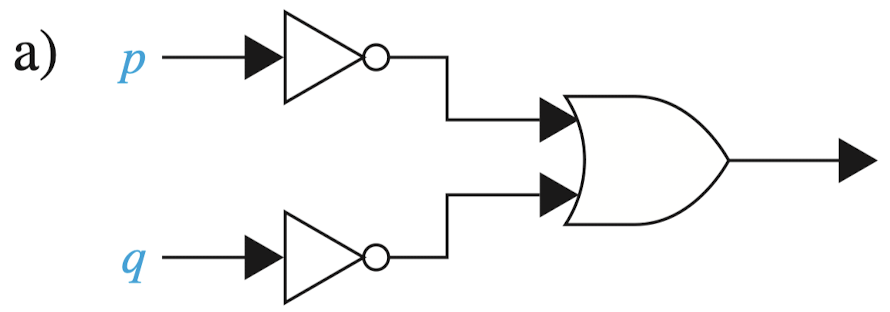
\includegraphics[width=0.35\linewidth]{Discrete Mathematics and its Applications, 8th Edition/Chapter 1 Logic and Proofs/Section 1.2 Applications of Propositional Logic/Exercise 44-a.png}
\end{figure}

\begin{figure}[h]
\centering
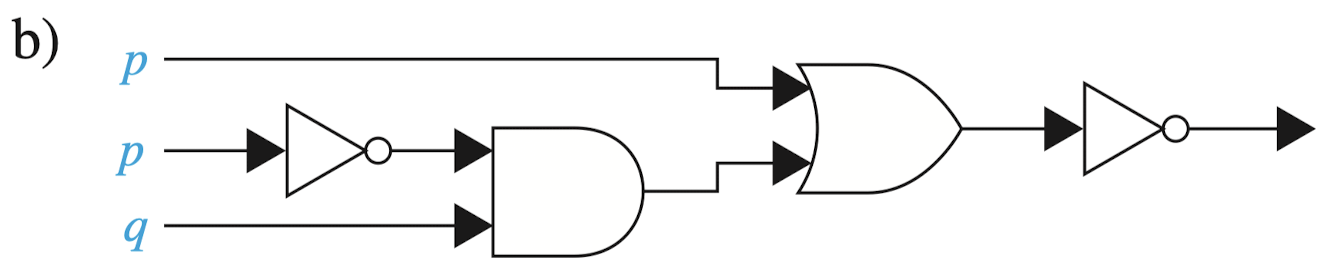
\includegraphics[width=0.5\linewidth]{Discrete Mathematics and its Applications, 8th Edition/Chapter 1 Logic and Proofs/Section 1.2 Applications of Propositional Logic/Exercise 44-b.png}
\end{figure}

\noindent
\textbf{Solution:}
\begin{enumerate}
    \item[\textbf{a)}] \(\lnot p \lor \lnot q\)
    \item[\textbf{b)}] \(\lnot(p \lor (\lnot p \land q))\)
\end{enumerate}

\section*{Exercise 45}
Find the output of each of these combinatorial circuits.

\begin{figure}[h]
\centering
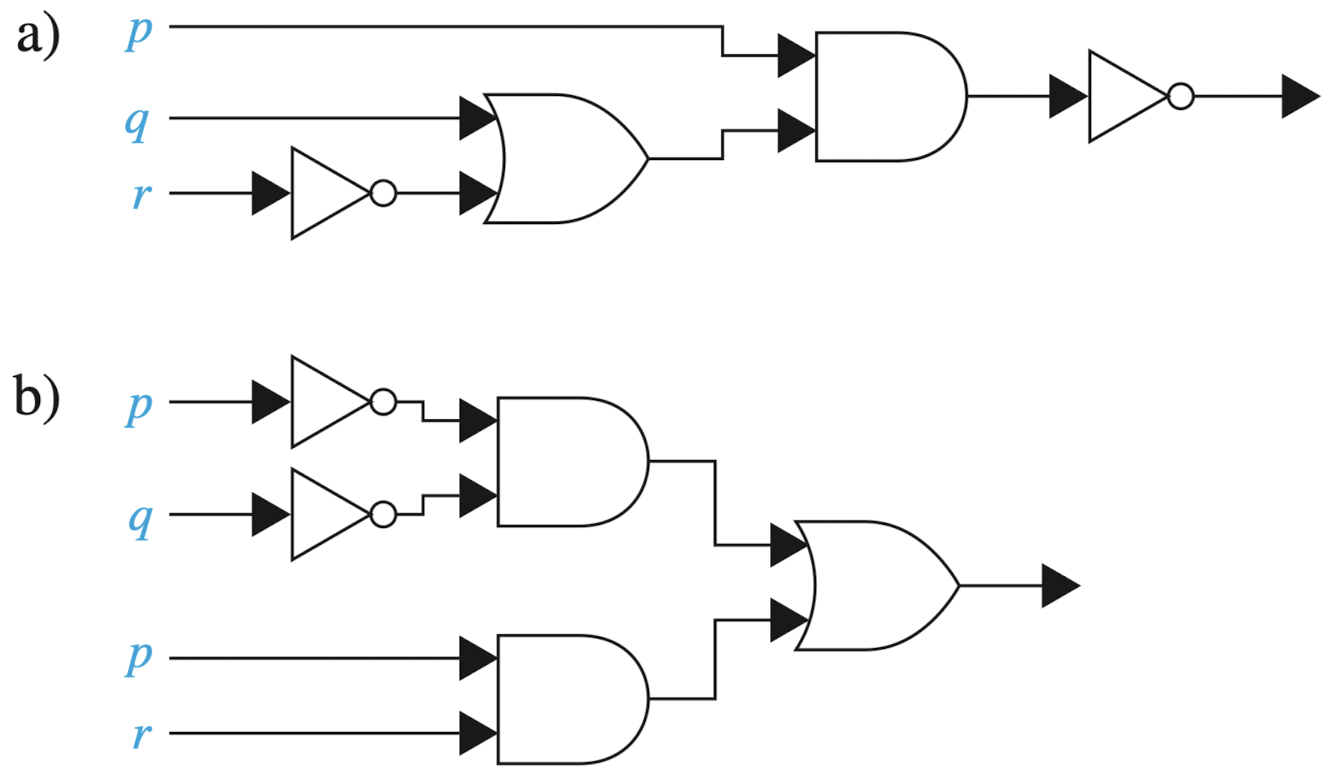
\includegraphics[width=0.5\linewidth]{Discrete Mathematics and its Applications, 8th Edition/Chapter 1 Logic and Proofs/Section 1.2 Applications of Propositional Logic/Exercise 45.png}
\end{figure}

\noindent
\textbf{Solution:}
\begin{enumerate}
    \item[\textbf{a)}] \(\lnot (p \land (q \lor \lnot r))\)
    \item[\textbf{b)}] \((\lnot p \land \lnot q) \lor (p \land r)\)
\end{enumerate}

\section*{Exercise 46}
Construct a combinatorial circuit using inverters, OR gates, and AND gates that produces the output \((p \land \lnot r) \lor (\lnot q \land r)\) from input bits \(p\), \(q\), and \(r\).

\noindent
\textbf{Solution:}
\begin{figure}[ht]
\centering
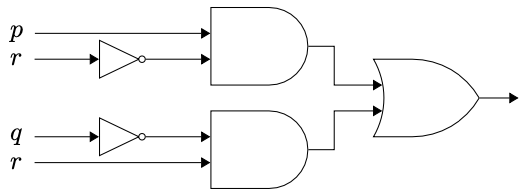
\includegraphics[width=0.5\linewidth]{Discrete Mathematics and its Applications, 8th Edition/Chapter 1 Logic and Proofs/Section 1.2 Applications of Propositional Logic/Exercise 46.png}
\end{figure}

\section*{Exercise 47}
Construct a combinatorial circuit using inverters, OR gates, and AND gates that produces the output \(((\lnot p \lor \lnot r) \land \lnot q) \lor (\lnot p \land (q \lor r))\) from the input bits \(p\), \(q\), and \(r\).

\noindent
\textbf{Solution:}
\begin{figure}[ht]
\centering
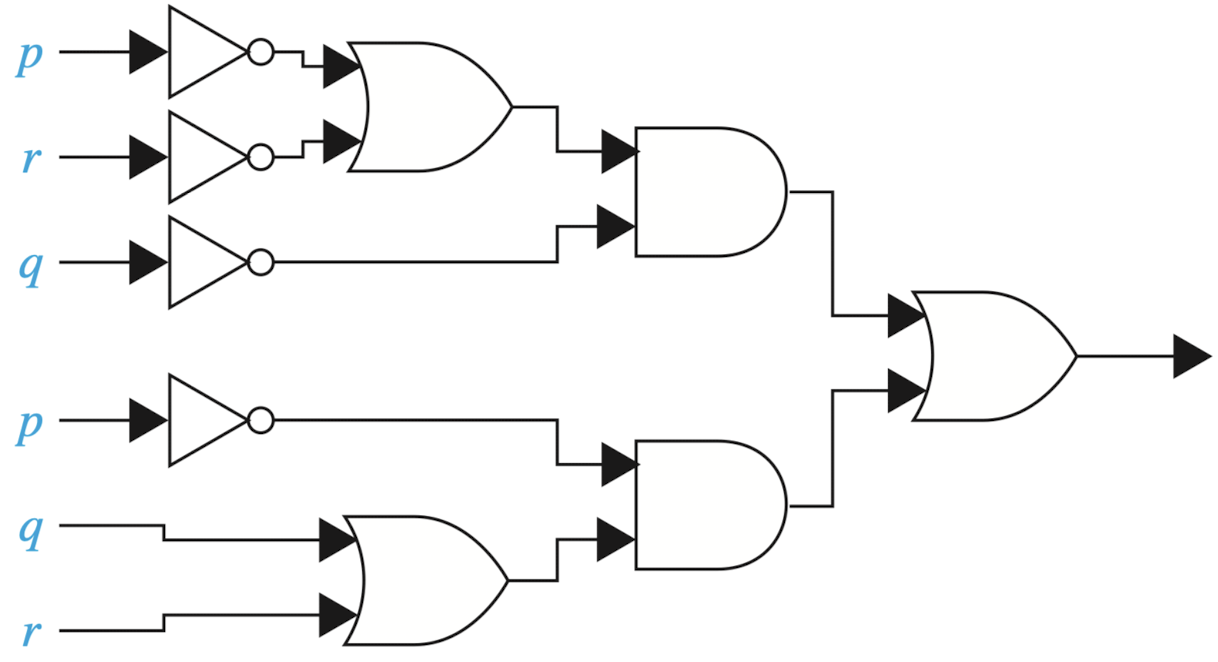
\includegraphics[width=0.5\linewidth]{Discrete Mathematics and its Applications, 8th Edition/Chapter 1 Logic and Proofs/Section 1.2 Applications of Propositional Logic/Exercise 47.png}
\end{figure}

\printbibliography

\end{document}